% ============================================================
% EMA AI - Owner Requirements Intelligence and Revit Evidence Review Framework
% External-facing technical publication
% Build: latexmk -pdf -interaction=nonstopmode -halt-on-error ema_ai_owner_requirements_intelligence_framework.tex
% ============================================================
\documentclass[10pt,letterpaper]{article}

% ------------------------------------------------------------
% Packages
% ------------------------------------------------------------
\usepackage[margin=0.58in]{geometry}
\usepackage[T1]{fontenc}
\usepackage[utf8]{inputenc}
\usepackage{lmodern}
\usepackage{microtype}
\usepackage{xcolor}
\usepackage{array}
\usepackage{tabularx}
\usepackage{booktabs}
\usepackage{longtable}
\usepackage{enumitem}
\usepackage[most]{tcolorbox}
\usepackage{fancyhdr}
\usepackage{lastpage}
\usepackage{hyperref}
\usepackage[strings]{underscore}
\usepackage{titlesec}
\usepackage{colortbl}
\usepackage{tikz}
\usepackage{amsmath}
\usepackage{caption}
\usetikzlibrary{arrows.meta,positioning,shapes.geometric}

% ------------------------------------------------------------
% Page setup
% ------------------------------------------------------------
\pagestyle{fancy}
\fancyhf{}
\renewcommand{\headrulewidth}{0pt}
\fancyfoot[L]{\footnotesize EMA AI - Owner Requirements Intelligence Framework}
\fancyfoot[C]{\footnotesize External-facing technical framework}
\fancyfoot[R]{\footnotesize Page \thepage\ of \pageref{LastPage}}

\hypersetup{
  colorlinks=true,
  linkcolor=emaNavy,
  urlcolor=emaNavy,
  citecolor=emaNavy
}

% ------------------------------------------------------------
% Color palette
% ------------------------------------------------------------
\definecolor{emaBlue}{HTML}{2563EB}
\definecolor{emaBlueDark}{HTML}{1D4ED8}
\definecolor{emaNavy}{HTML}{0F172A}
\definecolor{emaSlate}{HTML}{334155}
\definecolor{emaText}{HTML}{1E293B}
\definecolor{emaMuted}{HTML}{64748B}
\definecolor{emaLine}{HTML}{D8E2EE}
\definecolor{emaSoft}{HTML}{F8FAFC}
\definecolor{emaSoft2}{HTML}{F1F5F9}
\definecolor{emaGreen}{HTML}{15803D}
\definecolor{emaGreenBg}{HTML}{DCFCE7}
\definecolor{emaRed}{HTML}{B91C1C}
\definecolor{emaRedBg}{HTML}{FEE2E2}
\definecolor{emaAmber}{HTML}{B45309}
\definecolor{emaAmberBg}{HTML}{FEF3C7}
\definecolor{emaPurple}{HTML}{6D28D9}
\definecolor{emaPurpleBg}{HTML}{EDE9FE}
\definecolor{emaGrayBg}{HTML}{F1F5F9}
\definecolor{guardrailBlue}{HTML}{EFF6FF}
\definecolor{guardrailBorder}{HTML}{BFDBFE}
\definecolor{accentGray}{HTML}{CBD5E1}

% ------------------------------------------------------------
% Global style
% ------------------------------------------------------------
\renewcommand{\familydefault}{\sfdefault}
\setlength{\parindent}{0pt}
\setlength{\parskip}{4.5pt}
\setlength{\tabcolsep}{4.2pt}
\renewcommand{\arraystretch}{1.12}
\setlist[itemize]{leftmargin=1.15em,itemsep=2pt,topsep=2pt}
\setlist[enumerate]{leftmargin=1.35em,itemsep=2pt,topsep=2pt}
\setlength{\emergencystretch}{2em}
\sloppy

\titleformat{\section}{\Large\bfseries\color{emaNavy}}{}{0em}{}
\titlespacing{\section}{0pt}{15pt}{6pt}
\titleformat{\subsection}{\normalsize\bfseries\color{emaNavy}}{}{0em}{}
\titlespacing{\subsection}{0pt}{9pt}{4pt}
\titleformat{\subsubsection}{\small\bfseries\color{emaSlate}}{}{0em}{}
\titlespacing{\subsubsection}{0pt}{7pt}{3pt}

\tcbset{
  enhanced,
  boxrule=0.6pt,
  arc=3mm,
  left=8pt,
  right=8pt,
  top=7pt,
  bottom=7pt,
  colback=white,
  colframe=emaLine,
  breakable
}

% ------------------------------------------------------------
% Helpers
% ------------------------------------------------------------
\newcommand{\muted}[1]{\textcolor{emaMuted}{#1}}
\newcommand{\strong}[1]{\textbf{\textcolor{emaNavy}{#1}}}
\newcommand{\smalllabel}[1]{{\scriptsize\textcolor{emaMuted}{\MakeUppercase{#1}}}}
\newcommand{\code}[1]{\texttt{#1}}
\newcommand{\codepath}[1]{\path{#1}}
\newcommand{\flowarrow}{\ensuremath{\;\boldsymbol{\rightarrow}\;}}

\newcommand{\badge}[3]{%
  \tcbox[on line,colback=#2,colframe=#2,boxrule=0pt,arc=2mm,left=5pt,right=5pt,top=2pt,bottom=2pt]{%
    \scriptsize\textbf{\textcolor{#3}{#1}}}}
\newcommand{\metbadge}{\badge{Met}{emaGreenBg}{emaGreen}}
\newcommand{\notmetbadge}{\badge{Not Met}{emaRedBg}{emaRed}}
\newcommand{\reviewbadge}{\badge{Needs Human Review}{emaAmberBg}{emaAmber}}
\newcommand{\insufficientbadge}{\badge{Insufficient Model Data}{emaPurpleBg}{emaPurple}}
\newcommand{\nabadge}{\badge{Not Applicable}{emaGrayBg}{emaSlate}}
\newcommand{\manualbadge}{\badge{Manual}{emaGrayBg}{emaSlate}}
\newcommand{\hybridbadge}{\badge{Hybrid}{emaBlueDark!10}{emaBlueDark}}

\newcommand{\guardrailbox}[1]{%
\begin{tcolorbox}[colback=guardrailBlue,colframe=guardrailBorder,boxrule=0.6pt,arc=2mm,
  left=10pt,right=10pt,top=8pt,bottom=8pt]
\small #1
\end{tcolorbox}}

\newcommand{\keyconcept}[1]{%
\begin{tcolorbox}[colback=emaSoft,borderline west={3pt}{0pt}{emaBlue}]
\small #1
\end{tcolorbox}}

\tikzset{
  flowblock/.style={rectangle,draw=emaNavy!55,fill=emaSoft,rounded corners=2pt,
    minimum width=2.85cm,minimum height=0.78cm,text width=2.55cm,align=center,font=\footnotesize},
  flowwide/.style={rectangle,draw=emaNavy!55,fill=emaSoft,rounded corners=2pt,
    minimum width=3.35cm,minimum height=0.78cm,text width=3.10cm,align=center,font=\footnotesize},
  flowdecision/.style={diamond,draw=emaAmber!55,fill=emaAmberBg,aspect=1.9,
    inner sep=1.5pt,text width=2.25cm,align=center,font=\footnotesize},
  flowresult/.style={rectangle,draw=emaGreen!60,fill=emaGreenBg,rounded corners=2pt,
    minimum width=2.85cm,minimum height=0.78cm,text width=2.55cm,align=center,font=\footnotesize},
  arrow/.style={->,>=Stealth,thick}
}

% ------------------------------------------------------------
% Document
% ------------------------------------------------------------
\begin{document}
\color{emaText}

% ============================================================
% Cover page
% ============================================================
\thispagestyle{empty}
\begin{tcolorbox}[colback=white,colframe=emaNavy,boxrule=1.5pt,arc=5mm,
  left=20pt,right=20pt,top=28pt,bottom=28pt]
\begin{center}
  \vspace{4pt}
  {\Huge\bfseries\textcolor{emaNavy}{EMA AI}}\\[2pt]
  {\Huge\bfseries\textcolor{emaNavy}{Owner Requirements Intelligence}}\\[2pt]
  {\Huge\bfseries\textcolor{emaNavy}{and Revit Evidence Review Framework}}\\[12pt]
  {\Large\textcolor{emaMuted}{Deterministic review architecture for owner requirements, evidence alignment, and report-grounded AI assistance}}\\[16pt]
  {\normalsize\textcolor{emaSlate}{Version 1.0 \hspace{10pt} June 9, 2026}}\\[16pt]
  \begin{tcolorbox}[colback=emaSoft,colframe=emaLine,boxrule=0.5pt,arc=2mm,
    left=14pt,right=14pt,top=8pt,bottom=8pt]
    {\small\itshape\textcolor{emaMuted}{External-facing technical publication for EMA, Broadleaf, BIM/VDC managers, discipline leads, and Shokworks leadership. This document is descriptive, not a compliance certificate.}}
  \end{tcolorbox}
  \vspace{10pt}
  {\footnotesize\textcolor{emaMuted}{EMA AI is an Engineering Intelligence / Deliverable Readiness platform. It is not a generic chatbot and it is not a final compliance authority.}}\\[4pt]
  {\footnotesize\textcolor{emaMuted}{Revit Export \flowarrow FastAPI Ingestion \flowarrow PostgreSQL \flowarrow Deterministic Rules \flowarrow Evidence Review \flowarrow Report \flowarrow Ask EMA AI}}
\end{center}
\end{tcolorbox}

\vfill
\begin{tcolorbox}[colback=emaSoft2,colframe=emaLine,arc=2mm]
\small\textbf{Confidentiality / use note:} This document is intended for controlled external review and project alignment. It excludes secrets, credentials, private customer paths, and internal debugging language. It also avoids claims of automatic certification or autonomous engineering approval.
\end{tcolorbox}

\newpage
\tableofcontents
\newpage

% ============================================================
% 1. Executive summary
% ============================================================
\section{Executive Summary}

EMA AI is a Revit-first engineering intelligence workflow for reviewing owner requirements against model evidence, drawings, specifications, and human review paths. The system helps a design team answer a practical question: which requirements appear supported by current evidence, which are missing or ambiguous, which require human verification, and what should be done next.

\begin{tcolorbox}[colback=emaSoft]
\strong{Core trust model}
\begin{itemize}
  \item PostgreSQL is the official source of truth for the backend stack.
  \item The readiness engine is deterministic.
  \item LLMs explain, search, and draft suggestions, but do not decide official readiness or compliance.
  \item Candidate evidence is not accepted evidence until a reviewer accepts it.
  \item Revit-first review is the designer-facing path; dashboard sync is optional.
\end{itemize}
\end{tcolorbox}

EMA AI is intentionally conservative. It separates direct closing evidence from supporting context, surfaces missing evidence clearly, and pushes ambiguous, specification-driven, manual, or field-execution requirements toward human review instead of guessing.

\keyconcept{\strong{Positioning:} EMA AI is an Engineering Intelligence / Deliverable Readiness platform. It is not only a Revit QA/QC tool, and it is not a generic chatbot.}

% ============================================================
% 2. Product architecture context
% ============================================================
\section{Product Architecture Context}

The product is organized around a Revit-first data path:

\begin{center}
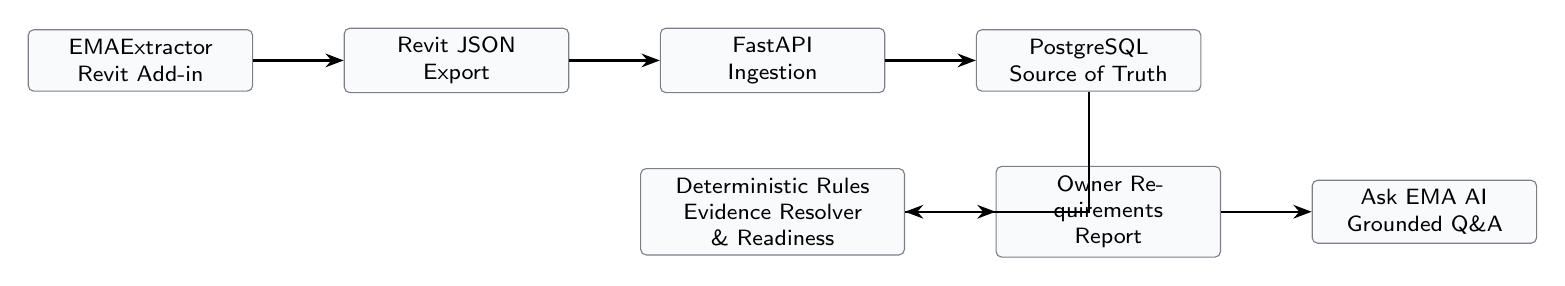
\begin{tikzpicture}[node distance=0.95cm and 1.15cm]
  \node[flowblock] (revit) {EMAExtractor\\Revit Add-in};
  \node[flowblock, right=of revit] (export) {Revit JSON\\Export};
  \node[flowblock, right=of export] (backend) {FastAPI\\Ingestion};
  \node[flowblock, right=of backend] (db) {PostgreSQL\\Source of Truth};
  \node[flowwide, below=of backend] (engine) {Deterministic Rules\\Evidence Resolver \& Readiness};
  \node[flowblock, right=of engine] (report) {Owner Requirements\\Report};
  \node[flowblock, right=of report] (ask) {Ask EMA AI\\Grounded Q\&A};
  \draw[arrow] (revit) -- (export);
  \draw[arrow] (export) -- (backend);
  \draw[arrow] (backend) -- (db);
  \draw[arrow] (db) |- (engine);
  \draw[arrow] (engine) -- (report);
  \draw[arrow] (report) -- (ask);
\end{tikzpicture}
\end{center}

Two distinct readiness layers exist in the repository:

\begin{table}[!h]
\centering
\small
\caption{Readiness layers in the current repository truth}\label{tab:readiness-layers}
\resizebox{\linewidth}{!}{%
\begin{tabular}{p{1.55in}p{1.65in}p{2.2in}p{1.8in}}
\toprule
\textbf{Layer} & \textbf{Where it lives} & \textbf{Primary formula} & \textbf{Role} \\
\midrule
\shortstack[l]{Report-side\\readiness} & ScoreCalculator & \shortstack[l]{40\% requirement coverage + 25\% evidence coverage\\+ 20\% QA/QC health + 10\% drawing/spec coverage\\+ 5\% sync freshness} & Local heuristic for preview surfaces. \\
\shortstack[l]{Backend readiness\\snapshot} & readiness/scoring.py & \shortstack[l]{50\% requirement coverage + 30\% QA/QC health\\+ 20\% sync freshness} & Official dashboard score and persisted snapshot. \\
\bottomrule
\end{tabular}
}
\end{table}

\keyconcept{\strong{Repo truth note:} the user-facing framework should describe both readiness layers. The backend readiness snapshot is the official dashboard path, while the Revit report can also display richer local heuristics.}

% ============================================================
% 3. EMAExtractor workflow
% ============================================================
\section{EMAExtractor Revit Add-in Workflow}

The Revit add-in is the designer entry point. Its ribbon is organized around four panels:

\begin{table}[!h]
\centering
\small
\caption{EMAExtractor ribbon structure}\label{tab:ribbon}
\begin{tabularx}{\linewidth}{p{1.55in}p{1.7in}>{\raggedright\arraybackslash}X p{1.45in}}
\toprule
\textbf{Panel} & \textbf{Commands} & \textbf{Purpose} & \textbf{Output} \\
\midrule
Owner Requirements Workflow & Open Workflow, Load Requirements, Sync Model Data, Run Check & Load a project, bind requirements, export model evidence, and execute the deterministic comparison workflow. & Report-ready evidence package. \\
Report & Report Navigator, Open Browser, Export PDF, Copy Summary & Open the latest report, print/export it, or copy a condensed summary. & HTML/PDF summary surfaces. \\
Ask EMA AI & Ask Report, Explain Issue & Ask grounded questions about the loaded report and selected issue. & Report-grounded responses and citations. \\
Support & Diagnostics, Settings, Dashboard & Inspect connection state, configure environment profile, and open the optional dashboard. & Diagnostics and navigation. \\
\bottomrule
\end{tabularx}
\end{table}

\subsection{Workflow path}

\begin{enumerate}
  \item Load the owner requirements workbook into the project context.
  \item Sync the current Revit model to export structured evidence.
  \item Run the deterministic comparison engine.
  \item Generate the HTML owner requirements report.
  \item Open the report in the navigator or browser fallback.
  \item Ask EMA AI against the loaded report context when needed.
\end{enumerate}

\subsection{Relevant command behavior}

\begin{table}[!h]
\centering
\small
\caption{Key add-in commands and behavior}\label{tab:addin-commands}
\begin{tabularx}{\linewidth}{p{2.15in}p{1.65in}X}
\toprule
\textbf{Command} & \textbf{Implementation path} & \textbf{Behavior} \\
\midrule
\codepath{OpenEmaPanelCommand} & Dashboard & Opens the modeless dashboard window. \\
\codepath{LoadRequirementsCommand} & RequirementsReadiness & Loads the workbook and prepares normalized requirements. \\
\codepath{SyncModelDataCommand} & SyncExport & Runs the export pipeline and captures model evidence. \\
\codepath{CheckRequirementsCommand} & RequirementsReadiness & Executes the deterministic owner-requirements comparison. \\
\codepath{OpenReportNavigatorCommand} & Reports & Opens the latest HTML report in the Revit-native navigator. \\
\codepath{OpenLastRequirementReportCommand} & RequirementsReadiness & Opens the newest report in the default browser. \\
\codepath{AskAboutReportCommand} and \codepath{ExplainSelectedIssueCommand} & Ai & Launch Ask EMA AI with report-grounded context. \\
\codepath{DiagnosticsCommand} and \codepath{SettingsCommand} & Settings & Show support, connection, and environment state. \\
\bottomrule
\end{tabularx}
\end{table}

\subsection{Navigation and fallback}

`EmaReportNavigatorWindow` is the main report surface in Revit. It can:

\begin{itemize}
  \item Load the latest report automatically by scanning report locations.
  \item Open a manually selected report.
  \item Render the report in WebView2 when available.
  \item Fall back to the system browser if WebView2 is unavailable or navigation fails.
  \item Keep Ask EMA AI grounded in the loaded HTML report data.
  \item Expose separate tabs for Report, Ask EMA AI, Taxonomy Matrix, and AI Audit.
\end{itemize}

\begin{tcolorbox}[colback=emaSoft]
\strong{Boundary statement:} the add-in prepares and reviews evidence. It does not parse PDFs as an authoritative source of truth, and it does not approve official compliance.
\end{tcolorbox}

% ============================================================
% 4. Data sources and intake
% ============================================================
\section{Data Sources and Intake}

The report pipeline consumes several source types. Some are authoritative inputs; others are supporting context or review artifacts.

\begin{longtable}{p{1.7in}p{1.35in}p{1.85in}p{1.9in}}
\caption{Primary intake sources and their role in the workflow}\label{tab:data-sources}\\
\toprule
\textbf{Source} & \textbf{Role} & \textbf{Typical fields} & \textbf{Notes} \\
\midrule
\endhead
Owner Requirements workbook & Authoritative input & `source_row`, worksheet, discipline, requirement text, category, status, links, resource & Ingested from Excel and normalized into requirement records. \\
Revit JSON export & Authoritative input for model evidence & element ID, unique ID, category, family, type, level, instance/type parameters & Produced by EMAExtractor and consumed by deterministic rules. \\
Model elements & Supporting evidence & category, family, type, level, parameter values & Used for evidence candidates and evidence alignment. \\
Drawings and specifications & Supporting or closing evidence & sheet number, spec section, title, page references & Important for drawing/spec/manual requirement types. \\
Manual reviewer input & Closing or adjudicating evidence & review notes, reviewed_by, reviewed_at, review status & Promotes or rejects evidence candidates. \\
Hidden report context JSON & Machine-readable report payload & summary counts, key issues, per-requirement details, AI hints & Embedded inside the HTML report for offline grounded Q\&A. \\
\bottomrule
\end{longtable}

\subsection{Exported Revit evidence}

The current export path carries:

\begin{itemize}
  \item Element identity: `unique_id` and numeric element ID.
  \item Structural placement: category, family, type, and level.
  \item Parameter stores: instance parameters and type parameters.
  \item Model metadata: export ID, sync time, and source project/model context.
\end{itemize}

\subsection{Supporting but not authoritative}

Context such as category, family, type, and level often helps narrow the search, but it does not automatically prove that a high-risk requirement is met. This distinction is central to the system design.

\guardrailbox{\strong{Relevant model context is not the same as direct closing evidence.} Category, family, type, or level may indicate scope, but they do not close manufacturer, controls, installation method, code, or field-execution requirements unless the requirement type explicitly allows that evidence profile.}

% ============================================================
% 5. Requirement normalization
% ============================================================
\section{Owner Requirement Normalization}

Workbook rows become structured owner requirements before any evidence comparison occurs. The normalized record preserves auditability and client binding.

\begin{longtable}{p{1.5in}p{1.85in}p{2.0in}p{1.4in}}
\caption{Normalization fields used by the repo}\label{tab:normalization}\\
\toprule
\textbf{Normalized field} & \textbf{Meaning} & \textbf{Typical source} & \textbf{Why it matters} \\
\midrule
\endhead
`source_row` & Original workbook row number & Excel row index & Preserves traceability to the source workbook. \\
`source_worksheet` & Worksheet name & Workbook tab name & Keeps discipline and section context visible. \\
`discipline` & Controlled discipline label & Explicit or inferred value & Drives routing and scope filtering. \\
`requirement_text` & Canonical requirement statement & Workbook requirement text & Primary semantic input to the classifier. \\
`category` & High-level requirement context & Workbook or inference & Guides taxonomy and evidence scope. \\
`owner_status` & Source workbook status & Client workbook field & Preserves the owner-side label without treating it as official readiness. \\
`is_actionable` & Checkability flag & Deterministic loader logic & Non-actionable rows are excluded from scoring. \\
`is_active` & Current applicability flag & Requirement ingestion state & Prevents retired rows from driving readiness. \\
`content_hash` & Stable fingerprint & Loader hash & Supports de-duplication and change detection. \\
\bottomrule
\end{longtable}

\subsection{Actionability logic}

Rows that behave as links, references, or documentation pointers are marked non-actionable and removed from readiness scoring. The system is designed to evaluate requirements, not to score reference rows.

\subsection{Normalization result}

After normalization, the engine can consistently evaluate:

\begin{itemize}
  \item project and client binding,
  \item discipline and scope filtering,
  \item row-level evidence alignment,
  \item requirement-type classification,
  \item status and next-action assignment.
\end{itemize}

% ============================================================
% 6. Requirement classification and taxonomy
% ============================================================
\section{Requirement Classification and Taxonomy}

The classifier maps each requirement into a semantic type that drives evidence expectations, validation type, and guardrails. The taxonomy is conservative: it tries to prevent false Met assignments by demanding the right evidence profile for the requirement intent.

\begin{longtable}{p{1.15in}p{1.0in}p{1.45in}p{1.45in}p{1.0in}}
\caption{Representative requirement taxonomy families}\\
\toprule
\textbf{Family} & \textbf{Typical validation} & \textbf{What model can prove} & \textbf{What model cannot prove} & \textbf{Risk level} \\
\midrule
\endhead
Electrical presence and circuiting & Model & Equipment presence, panel, circuit, voltage, load metadata & Compliance with load calcs, AIC, phase balancing & Medium \\
Lighting and lighting controls & Model or Specification & Fixture presence, circuit/panel, control device presence & Control scheme completeness, zoning logic & Medium to high \\
Mechanical equipment and performance & Model or Specification & Equipment presence, family/type, level, manufacturer metadata when populated & Controls, performance, installation method, field work & High \\
Plumbing fixtures, piping, and accessories & Model or Hybrid & Pipe/fitting/accessory presence, size, material, zone & Coverage rules, product constraints, field verification & High \\
Technology, security, fire alarm, AV & Model or Hybrid & Device presence, panel, circuit, zone, level & Programming, cable type/color, system logic, spec limits & High \\
Documents, approvals, code, closeout & Manual or Specification & Very little without external documents & Approval status, testing, O\&M, code interpretation & Very high \\
\bottomrule
\end{longtable}

\subsection{Canonical requirement-type inventory}

The repository taxonomy JSON defines the full semantic inventory below. ``Current'' means the type exists in the present classifier. ``Planned'' means it is recommended by the canonical taxonomy but not yet fully surfaced in the current runtime classifier.

\small
\begin{longtable}{p{3.25in}p{1.05in}p{1.35in}}
\caption{Canonical requirement-type inventory}\\
\toprule
\textbf{Requirement type} & \textbf{State} & \textbf{Model checkability} \\
\midrule
\endhead
\codepath{grounding_bonding_conductors} & Current & partial \\
\codepath{plumbing_hose_bibb_rpz_valves} & Current & partial \\
\codepath{manufacturer_product_spec_submittal} & Current & never \\
\codepath{identification_labeling_nameplate} & Current & never \\
\codepath{drawing_spec_manual_owner_approval} & Current & never \\
\codepath{field_execution_demolition_protection} & Current & never \\
\codepath{panel_circuit_power} & Current & partial \\
\codepath{outlets_receptacles_devices} & Current & partial \\
\codepath{technology_low_voltage_security_fire_alarm} & Current & partial \\
\codepath{conduit_raceway} & Current & never for size \\
\codepath{controls_bms_bas_contactors_relays} & Current & never \\
\codepath{commissioning_testing_om_training} & Current & never \\
\codepath{mechanical_equipment_coverage} & Current & partial \\
\codepath{level_location_mounting_placement} & Current & partial \\
\codepath{unknown_ambiguous} & Current fallback & varies \\
\codepath{conduit_raceway_size_requirement} & Planned & never \\
\codepath{flexible_conduit_length_requirement} & Planned & never \\
\codepath{mechanical_controls_ddc_emcs} & Planned & never \\
\codepath{manufacturer_brand_restriction} & Planned & partial if parameter populated \\
\codepath{product_model_specification} & Planned & partial if parameter populated \\
\codepath{pipe_material_specification} & Planned & partial \\
\codepath{pipe_size_specification} & Planned & partial \\
\codepath{plumbing_fixture_model_specification} & Planned & partial \\
\codepath{fire_protection_sprinkler} & Planned & partial \\
\codepath{backfill_excavation_earthwork} & Planned & never \\
\codepath{demolition_existing_work} & Planned & never \\
\codepath{installation_method_execution} & Planned & never \\
\codepath{owner_approval_coordination} & Planned & never \\
\codepath{testing_inspection_startup} & Planned & never \\
\codepath{operation_maintenance_manual} & Planned & never \\
\codepath{attic_stock_spare_parts} & Planned & never \\
\codepath{engraving_labeling_finishing} & Planned & never \\
\codepath{storm_shelter_requirements} & Planned & partial \\
\codepath{kitchen_cafeteria_specialty} & Planned & partial \\
\codepath{gymnasium_specialty} & Planned & partial \\
\codepath{electrical_load_voltage_calculation} & Planned & partial \\
\codepath{lighting_control_scheme} & Planned & never \\
\bottomrule
\end{longtable}
\normalsize

\subsection{Repository taxonomy signals}

The classifier currently recognizes the following validation labels in code:

\begin{center}
\metbadge\hspace{6pt}\badge{Drawing}{emaAmberBg}{emaAmber}\hspace{6pt}\badge{Specification}{emaPurpleBg}{emaPurple}\hspace{6pt}\manualbadge\hspace{6pt}\hybridbadge
\end{center}

\subsection{Taxonomy matrix concept}

The report includes a Taxonomy Matrix tab so reviewers can see:

\begin{itemize}
  \item the inferred requirement type,
  \item expected categories and parameters,
  \item direct closing evidence,
  \item supporting context,
  \item false-positive risks,
  \item whether the requirement is actually model-closeable.
\end{itemize}

\keyconcept{\strong{Model-closeable is not a synonym for model-present.} A category match may be useful context, but it is not enough to close a requirement whose intent depends on product data, controls, drawings, or manual review.}

% ============================================================
% 7. Validation type framework
% ============================================================
\section{Validation Type Framework}

The repository uses five primary validation types in the add-in:

\begin{longtable}{p{1.2in}p{1.7in}p{2.1in}p{1.9in}}
\caption{Validation types and how they behave}\\
\toprule
\textbf{Type} & \textbf{Meaning} & \textbf{Typical evidence} & \textbf{Common closure rule} \\
\midrule
\endhead
Model & Evidence comes from Revit model data & category, family, type, parameters, level & Can close when direct evidence is complete. \\
Drawing & Evidence comes from sheet/detail context & sheet number, detail note, drawing reference & Usually requires review or sheet citation. \\
Specification & Evidence comes from spec or product criteria & product data, manufacturer, submittal, code text & Requires a direct spec or product reference. \\
Manual & Evidence needs human judgment or field verification & reviewer notes, field observation, owner approval & Does not close from model data alone. \\
Hybrid & A model component exists, but another source is still required & model plus drawing/spec/manual evidence & Requires both the model context and the external proof. \\
\bottomrule
\end{longtable}

\subsection{Customer-facing interpretation}

These labels are intentionally conservative. The system would rather return \textsc{Needs Human Review} than treat generic model context as proof.

\subsection{Not Model Closeable}

The codebase does not expose a separate enum value named `Not Model Closeable`, but the phrase is still useful as a customer-facing concept for requirements that cannot be safely closed from model evidence alone. In practice, such items usually resolve to Drawing, Specification, Manual, or Hybrid behavior.

% ============================================================
% 8. Evidence framework
% ============================================================
\section{Evidence Framework}

This is the core conceptual layer in the product. It keeps the difference between evidence, context, and review state explicit.

\begin{table}[!h]
\centering
\small
\caption{Evidence vocabulary used by the framework}\label{tab:evidence-framework}
\resizebox{\linewidth}{!}{%
\begin{tabular}{p{1.5in}p{2.45in}p{3.0in}}
\toprule
\textbf{Evidence term} & \textbf{Meaning} & \textbf{How the system treats it} \\
\midrule
Direct Closing Evidence & Evidence strong enough to close the requirement deterministically & Can support Met or compliant status when allowed. \\
Supporting Context & Evidence that narrows the search but does not prove the requirement & May contribute to scope or confidence, but not closure. \\
Candidate Evidence & A possible match generated by deterministic or AI-assisted review & Stays in candidate status until accepted. \\
Accepted Evidence & A reviewer has confirmed the evidence is valid & Can support covered or compliant status. \\
Rejected Evidence & A reviewer has explicitly rejected the candidate & Does not count as covered. \\
Missing Direct Evidence & The expected proof is absent from the model or documents & Drives Not Met, Needs Human Review, or Missing status. \\
Insufficient Evidence & The system cannot find enough structured proof to decide safely & Often maps to Insufficient Model Data. \\
\bottomrule
\end{tabular}
}
\end{table}

\begin{tcolorbox}[colback=emaSoft]
\strong{Evidence ladder}
\begin{center}
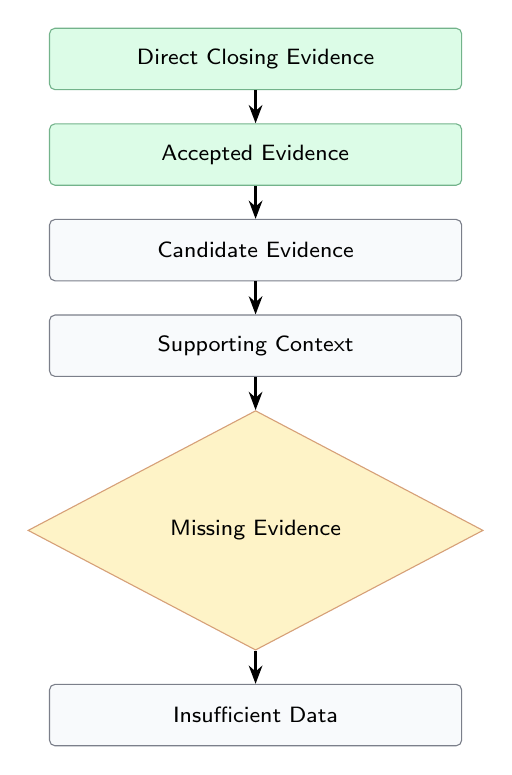
\begin{tikzpicture}[node distance=0.42cm]
  \node[flowresult, text width=5.0cm] (e1) {Direct Closing Evidence};
  \node[flowresult, below=of e1, text width=5.0cm] (e2) {Accepted Evidence};
  \node[flowblock, below=of e2, text width=5.0cm] (e3) {Candidate Evidence};
  \node[flowblock, below=of e3, text width=5.0cm] (e4) {Supporting Context};
  \node[flowdecision, below=of e4, text width=5.0cm] (e5) {Missing Evidence};
  \node[flowblock, below=of e5, text width=5.0cm] (e6) {Insufficient Data};
  \draw[arrow] (e1) -- (e2);
  \draw[arrow] (e2) -- (e3);
  \draw[arrow] (e3) -- (e4);
  \draw[arrow] (e4) -- (e5);
  \draw[arrow] (e5) -- (e6);
\end{tikzpicture}
\end{center}
\end{tcolorbox}

\subsection{Required guardrails}

\guardrailbox{\strong{Candidate evidence never counts as covered until accepted by a reviewer.}}

\guardrailbox{\strong{Category, family, type, or level alone should not close high-risk requirements unless the requirement type explicitly allows that evidence profile.}}

\guardrailbox{\strong{Relevant model context is not the same as direct closing evidence.}}

% ============================================================
% 9. Model evidence resolver
% ============================================================
\section{Model Evidence Resolver}

The deterministic resolver is the mechanism that turns Revit element rows into evidence candidates. It is intentionally simple, reproducible, and bounded.

\subsection{Intent patterns}

The resolver classifies each requirement into one of a small set of intent patterns such as:

\begin{itemize}
  \item electrical panel / circuit / power,
  \item lighting,
  \item mechanical equipment,
  \item plumbing fixtures and accessories,
  \item technology and low-voltage devices,
  \item generic model fallback.
\end{itemize}

\subsection{Scoring model}

The current scoring formula in `model_evidence_resolver.py` is:

\[
\text{score} = 0.35\,C + 0.15\,K + 0.15\,P + 0.10\,T + 0.05\,L
\]

where:

\begin{itemize}
  \item $C$ = category match,
  \item $K$ = keyword match in element text,
  \item $P$ = required parameter presence,
  \item $T$ = requirement category appears in the element text,
  \item $L$ = level exists.
\end{itemize}

The score is capped at 1.0. Candidates meeting the low threshold of 0.40 are retained; stronger candidates above 0.65 are treated as higher confidence but still not auto-approved.

\begin{longtable}{p{1.8in}p{1.9in}p{2.0in}}
\caption{Candidate generation thresholds}\label{tab:candidate-thresholds}\\
\toprule
\textbf{Threshold} & \textbf{Value} & \textbf{Behavior} \\
\midrule
\endhead
Low threshold & 0.40 & Candidate is eligible to be created or retained. \\
High threshold & 0.65 & Candidate is strong enough to surface prominently, but still requires review. \\
No-auto-approve rule & Always on & Candidate evidence remains `needs_review` until acceptance. \\
\bottomrule
\end{longtable}

\subsection{Why the resolver exists}

The resolver creates a structured bridge between model export rows and owner requirements. It helps the team:

\begin{itemize}
  \item identify likely matches,
  \item rank candidate evidence,
  \item avoid scanning the full model repeatedly,
  \item keep evidence candidates separate from official compliance,
  \item preserve reviewer judgment in the loop.
\end{itemize}

\subsection{Resolver output}

When a candidate is created, the repository stores:

\begin{itemize}
  \item `evidence_type = model`,
  \item `evidence_status = needs_review`,
  \item `review_status = candidate`,
  \item `source_ref = model:<unique_id>`,
  \item metadata with scoring breakdown, matched intent, and matched parameters.
\end{itemize}

\keyconcept{\strong{Deterministic rule:} candidate evidence stays at candidate status until a reviewer explicitly accepts or rejects it.}

% ============================================================
% 10. Status logic
% ============================================================
\section{Status Logic}

The add-in and backend use related but not identical status vocabularies. The report should explain the mapping clearly instead of collapsing them into a single label.

\begin{longtable}{p{1.35in}p{1.55in}p{1.75in}p{2.1in}}
\caption{Status decision table}\label{tab:status-logic}\\
\toprule
\textbf{Evidence condition} & \textbf{Backend normalized status} & \textbf{Report label} & \textbf{Reviewer action} \\
\midrule
\endhead
Accepted evidence with supporting compliance row & \codepath{compliant} / \codepath{covered} & Met & Usually no immediate action unless the requirement changes. \\
Rejected evidence or clear missing proof & \codepath{non_compliant} / \codepath{missing} & Not Met & Fix the model, documentation, or source evidence and rerun. \\
Candidate or needs-review evidence & \codepath{needs_review} / \codepath{needs_review} & Needs Human Review & Review and either accept, reject, or request more proof. \\
Requirement is outside the selected discipline or scope & \codepath{not_applicable} / \codepath{not_applicable} & Not Applicable & Confirm scope, then exclude or re-run the correct discipline. \\
No structured model evidence available & \codepath{missing} / \codepath{blocked} in some downstream contexts & Insufficient Model Data & Gather more model data or move to drawing/spec/manual review. \\
Blank or unreadable row & \codepath{not_evaluated} or human-review path & Needs Human Review & Repair the source row and rerun normalization. \\
\bottomrule
\end{longtable}

\subsection{Important backend distinctions}

The backend schemas distinguish between:

\begin{itemize}
  \item \codepath{requirement_compliance.status} with values such as \codepath{compliant}, \codepath{non_compliant}, \codepath{not_evaluated}, \codepath{not_applicable}, \codepath{needs_review},
  \item \codepath{requirement_evidence.evidence_status} with values such as \codepath{covered}, \codepath{missing}, \codepath{needs_review}, \codepath{blocked}, \codepath{not_applicable},
  \item \codepath{review_status} values such as \codepath{candidate}, \codepath{accepted}, \codepath{rejected}, \codepath{needs_review}, \codepath{none}.
\end{itemize}

\subsection{Natural language interpretation}

\begin{tcolorbox}[colback=emaSoft]
The repository never treats candidate evidence as official compliance. A candidate can inform a reviewer, but it cannot approve itself.
\end{tcolorbox}

% ============================================================
% 11. Readiness engine
% ============================================================
\section{Readiness Engine}

EMA AI has two deterministic readiness stories:

\subsection{Backend readiness snapshot}

The backend uses a simple weighted readiness formula:

\[
\text{Overall Readiness} = 0.50(\text{Requirement Coverage}) + 0.30(\text{QA/QC Health}) + 0.20(\text{Sync Freshness})
\]

This is the official dashboard path. In the backend service, requirement coverage is measured from actionable, applicable requirements; `not_applicable` items are excluded from the denominator.

\subsection{Report-side readiness metrics}

The Revit report can display a richer local heuristic:

\[
\begin{aligned}
\text{Report Readiness} &= 0.40(\text{Requirement Coverage}) + 0.25(\text{Evidence Coverage}) \\
&\quad + 0.20(\text{QA/QC Health}) + 0.10(\text{Drawing/Spec Coverage}) + 0.05(\text{Sync Freshness})
\end{aligned}
\]

This is useful for the local report view, but it should not be described as a separate compliance certification.

\subsection{What readiness means}

Readiness is a deliverable-health indicator, not a certificate. It is designed to show whether the team has enough covered owner requirements, enough healthy QA/QC, and enough sync freshness to move forward responsibly.

\begin{table}[!h]
\centering
\small
\caption{Readiness semantics}\label{tab:readiness-semantics}
\resizebox{\linewidth}{!}{%
\begin{tabular}{p{1.45in}p{1.95in}p{1.9in}p{1.7in}}
\toprule
\textbf{Concept} & \textbf{What it means} & \textbf{What it does not mean} & \textbf{Repo rule} \\
\midrule
Covered & \shortstack[l]{Officially satisfied\\in the active deterministic path} & \shortstack[l]{Not a guarantee of\\final project approval} & \shortstack[l]{Counted in coverage\\if applicable.} \\
Evaluated & \shortstack[l]{The requirement\\has been assessed} & Not necessarily covered & \shortstack[l]{Non-compliant items remain\\out of coverage.} \\
Candidate & \shortstack[l]{Potential evidence\\waiting for reviewer action} & Not evidence coverage & \shortstack[l]{Candidate does not\\count as covered.} \\
Not applicable & \shortstack[l]{Outside scope\\for the current review} & Not a failure & \shortstack[l]{Excluded from the\\applicable denominator.} \\
\bottomrule
\end{tabular}
}
\end{table}

\subsection{Trade readiness}

The backend also computes discipline-level trade readiness rows. Those rows summarize discipline-specific requirement totals, evaluated counts, missing requirements, needs-review counts, and open issues. If a project lacks linked requirements, the system can still show a model-health fallback, but that fallback is not official owner-requirements readiness.

\keyconcept{\strong{Covered does not equal evaluated, and evaluated does not always equal covered.} The repository explicitly preserves that difference.}

% ============================================================
% 12. Key Issue Score
% ============================================================
\section{Key Issue Score and Prioritization}

Key Issue Score is a prioritization score, not a compliance score. It exists to help teams focus on the highest-impact gaps first.

\subsection{Executable formula}

The current engine implements:

\[
\text{KeyIssueScore} = 0.30S + 0.20D + 0.20I + 0.15G + 0.10C + 0.05A
\]

where:

\begin{itemize}
  \item $S$ = status severity,
  \item $D$ = discipline relevance,
  \item $I$ = deliverable impact,
  \item $G$ = evidence gap,
  \item $C$ = confidence,
  \item $A$ = actionability.
\end{itemize}

The workflow service currently implements the following normalized inputs:

\begin{table}[!h]
\centering
\small
\caption{Key Issue Score components used by the engine}\label{tab:key-issue-components}
\begin{tabularx}{\linewidth}{p{1.4in}p{1.85in}>{\raggedright\arraybackslash}X}
\toprule
\textbf{Component} & \textbf{Current implementation} & \textbf{Meaning} \\
\midrule
Status severity & Not Met = 1.0; Insufficient Model Data = 0.75; Needs Human Review = 0.60; otherwise 0.0 & How urgent the status is by itself. \\
Discipline relevance & 1.0 (all issues) & All issues are discipline-relevant in the current implementation. \\
Deliverable impact & 0.9 & Reflects likely deliverable consequence. \\
Evidence gap & 1.0 for Not Met; 0.5 otherwise & Missing direct proof should rank higher than partial ambiguity. \\
Confidence & Result confidence value & Prevents low-confidence items from scoring the same as strong matches. \\
Actionability & 0.75 when a next action exists; 0.25 otherwise & Measures whether the issue has a clear route to resolution. \\
\bottomrule
\end{tabularx}
\end{table}

\subsection{Customer-facing interpretation}

The customer-facing story is straightforward:

\begin{itemize}
  \item a missing panel/circuit assignment should rank higher than a minor note,
  \item a controls or spec issue should rank higher than a generic context issue,
  \item an issue with a clear next action is easier to route and solve,
  \item confidence is a modifier, not a waiver.
\end{itemize}

\subsection{Difference from readiness}

\begin{tcolorbox}[colback=emaSoft]
\strong{Key Issue Score} answers \emph{what should we fix first?}  
\strong{Readiness} answers \emph{how healthy is the deliverable right now?}
\end{tcolorbox}

% ============================================================
% 13. Recommended actions
% ============================================================
\section{Recommended Actions and Next Best Action}

Next Best Action is the operational output of the rule engine. It translates the gap into an action the team can actually perform.

\begin{longtable}{p{1.55in}p{1.9in}p{2.65in}}
\caption{Action types surfaced by the repository}\\
\toprule
\textbf{Action type} & \textbf{Typical trigger} & \textbf{Example detail} \\
\midrule
\endhead
\codepath{assign_discipline} & A row needs routing to a discipline owner & Reassign to Electrical, Mechanical, Plumbing, Lighting, or Technology lead. \\
\codepath{attach_source} & The requirement needs a linked source document & Attach a drawing, specification, or source file citation. \\
\codepath{map_milestone} / \codepath{map_trade} & The requirement needs project-phase or discipline mapping & Bind the row to the correct milestone or trade scope. \\
\codepath{map_evidence_type} & The row needs a clearer evidence expectation & Mark the row as Model, Drawing, Specification, Manual, or Hybrid. \\
\codepath{link_evidence} / \codepath{review_evidence} & Candidate evidence exists & Accept, reject, or refine the candidate evidence. \\
\codepath{review_requirement} & The requirement is ambiguous or underclassified & Resolve the semantic type or rewrite the requirement text. \\
\codepath{evaluate_requirements} & The project needs a rerun after updates & Recompute the deterministic comparison and report. \\
\codepath{review_trade_gaps} & Discipline gaps are concentrated & Route to the relevant trade review owner. \\
\codepath{run_sync} & The model export is stale or missing & Refresh the Revit export and ingest again. \\
\codepath{review_issue_backlog} & High issue density is blocking readiness & Prioritize the open issue backlog before the next deliverable. \\
\bottomrule
\end{longtable}

\subsection{Action logic}

The engine tries to make the next step specific enough to be useful and conservative enough to avoid overclaiming. If the evidence is incomplete, the next action will often be review-oriented rather than closure-oriented.

\keyconcept{\strong{Actionability is part of prioritization, not proof.} A clear next step does not make the requirement compliant.}

% ============================================================
% 14. Owner Requirements report output structure
% ============================================================
\section{Owner Requirements Report Output Structure}

The HTML report generated by `OwnerRequirementHtmlReportGenerator` is the primary user-facing artifact. It is self-contained, uses embedded CSS and JavaScript, and does not rely on external assets.

\begin{longtable}{p{1.6in}p{2.8in}p{2.3in}}
\caption{Report sections and their purpose}\\
\toprule
\textbf{Section} & \textbf{Purpose} & \textbf{Current state} \\
\midrule
\endhead
Header and hero & Project name, model, requirements file, and active filter context & Current. \\
Filter bar and focus banner & Filter by discipline, status, and urgency & Current. \\
Executive summary & KPI cards and top-line health snapshot & Current. \\
Discipline allocation & Per-discipline breakdown and impact summary & Current. \\
Status and urgency legends & Semantic reference for report colors & Current. \\
Top overall issues & Key issue cards and urgency ranking & Current. \\
Issues by urgency & Grouped view of high-priority gaps & Current. \\
Discipline sections and requirement cards & Detailed row-level evidence review & Current. \\
Evidence and traceability & Element IDs, matched evidence, and rule traces & Current. \\
Ask EMA AI & Report-grounded question prompts & Current. \\
Report notes & No-overclaim disclaimer and review boundary & Current. \\
Taxonomy Matrix, AI Audit, Exports, Rules, Elements & Additional review/navigation tabs in the navigator surface & Current in the report navigator UI, with export details depending on report scope. \\
\bottomrule
\end{longtable}

\subsection{Machine-readable report context}

The HTML report embeds a hidden JSON payload at \code{\#ema-ai-report-context}. The navigator and Ask EMA AI surface read that payload directly for grounded answers and report-aware summaries.

\begin{tcolorbox}[colback=emaSoft]
\strong{Report-grounded question flow:} HTML report \flowarrow hidden JSON \flowarrow RAG context \flowarrow deterministic answer or provider-based answer \flowarrow cited response.
\end{tcolorbox}

% ============================================================
% 15. Hidden report context JSON
% ============================================================
\section{Hidden Report Context JSON}

The hidden JSON exists so the report can be machine-readable without exposing sensitive data externally or depending on a remote index.

\subsection{Why it exists}

\begin{itemize}
  \item It lets Ask EMA AI answer questions using the loaded report context.
  \item It lets the navigator parse the report offline or locally.
  \item It keeps the report self-contained and portable.
  \item It supports traceability without forcing a backend round-trip.
\end{itemize}

\subsection{Key fields in the current payload}

\begin{longtable}{p{1.65in}p{1.95in}p{3.05in}}
\caption{Hidden JSON fields emitted by the report generator}\\
\toprule
\textbf{Field} & \textbf{Source of truth} & \textbf{Description} \\
\midrule
\endhead
\codepath{schema_version} & Report generator & Payload version. \\
\codepath{report_metadata} & Report generator & Project, model, requirements file, scope, generated time, total requirements, model elements reviewed. \\
\codepath{summary_counts} & Requirement summary & Met, Not Met, Needs Human Review, Insufficient Model Data, Not Applicable counts. \\
\codepath{filter_context} & Current report view & Active discipline, status, urgency, visible counts, scores, and suggested questions. \\
\codepath{key_issues} & Key issue ranking & Ranked issue list including source row, title, urgency, evidence summary, action, confidence, key issue score, and score factors. \\
\codepath{requirement_results} & Per-row results & Full per-requirement detail including evidence traces, candidate scope, next action, status reason, and AI hints. \\
\codepath{ai_lookup_hints} & Per-row result helper & Search terms, evidence location, likely owner, suggested question, and element IDs. \\
\bottomrule
\end{longtable}

\subsection{Important row-level fields}

The current report payload exposes fields such as:

\begin{itemize}
  \item `requirement_id`
  \item `source_row`
  \item `source_worksheet`
  \item `discipline`
  \item `requirement_text`
  \item `requirement_type`
  \item `validation_type`
  \item `rule_applied`
  \item `evidence_alignment`
  \item `status`
  \item `urgency`
  \item `confidence`
  \item `next_best_action`
  \item `candidate_scope_valid`
  \item `full_model_fallback_used`
  \item `direct_closing_evidence`
  \item `supporting_context`
  \item `missing_direct_evidence`
  \item `matched_element_ids`
  \item `score_factors`
\end{itemize}

% ============================================================
% 16. Ask EMA AI and AI boundaries
% ============================================================
\section{Ask EMA AI and AI Boundaries}

The Ask EMA AI panel is not a general chatbot. It is a report-grounded assistant that answers from the loaded HTML report context.

\subsection{Provider chain}

The current model-selection logic supports:

\begin{enumerate}
  \item a deterministic built-in fallback,
  \item local Ollama models,
  \item OpenRouter,
  \item other OpenAI-compatible providers wired through the model configuration.
\end{enumerate}

The configuration loader searches for `opencode.json` and also maintains a fallback list that includes local and cloud options. The current fallback list in code includes Qwen 3.6 35B, Granite 4.1 30B, Gemma 4 26B, Claude Sonnet 4, and GPT-4.1 alongside the deterministic option.

\subsection{What Ask EMA AI can do}

\begin{itemize}
  \item explain requirement status, evidence, and reasoning,
  \item summarize key issues and next actions,
  \item answer row-specific or discipline-specific questions,
  \item cite requirement rows and element IDs when available,
  \item work offline with deterministic report logic when a model is unavailable.
\end{itemize}

\subsection{What Ask EMA AI must not do}

\begin{itemize}
  \item certify compliance,
  \item change official statuses,
  \item invent evidence,
  \item replace engineering review,
  \item make legal or contractual claims.
\end{itemize}

\guardrailbox{\strong{Ask EMA AI can explain the loaded report context, but it does not create final engineering approval.}}

\subsection{Grounding behavior}

The navigator builds a report-specific prompt from the hidden JSON payload and the current chat scope. If the selected model is unavailable or the answer cannot be produced reliably, the system falls back to deterministic report text rather than inventing a response.

% ============================================================
% 17. AI audit and taxonomy matrix
% ============================================================
\section{AI Audit and Taxonomy Matrix}

The Taxonomy Matrix and AI Audit tabs are review tools, not production claims. They help reviewers see whether a requirement type is well defined, whether the current classification is safe, and where tuning is needed.

\subsection{AI audit signals}

\begin{itemize}
  \item unknown or ambiguous requirement type detection,
  \item false Met risk detection,
  \item candidate scope warnings,
  \item generic next-action detection,
  \item narrative contradiction checks,
  \item missing direct evidence checks,
  \item taxonomy coverage gaps.
\end{itemize}

\subsection{Why this makes the report safer}

The audit layer is a control surface. It helps the team see where a rule is too broad, where a requirement needs a better type, and where a yes/no decision would be too risky.

\begin{longtable}{p{1.55in}p{2.5in}p{2.35in}}
\caption{Audit benefit matrix}\\
\toprule
\textbf{Audit check} & \textbf{What it catches} & \textbf{Why it matters} \\
\midrule
\endhead
Unknown type detection & Requirements that fall into fallback handling & Reveals taxonomy gaps. \\
False Met risk detection & Rows that appear supported but lack direct proof & Protects against overclaiming. \\
Candidate scope warnings & Candidate sets that are too broad or use full-model fallback & Prevents weak evidence from masquerading as closure. \\
Next action quality checks & Generic or unhelpful next steps & Improves reviewer usefulness. \\
Contradiction checks & Conflicting evidence or status narrative & Makes the report more trustworthy. \\
\bottomrule
\end{longtable}

% ============================================================
% 18. EMA tuning and human review loop
% ============================================================
\section{EMA Tuning and Human Review Loop}

The system is built to improve through reviewer feedback. Tuning is expected, not a failure.

\begin{center}
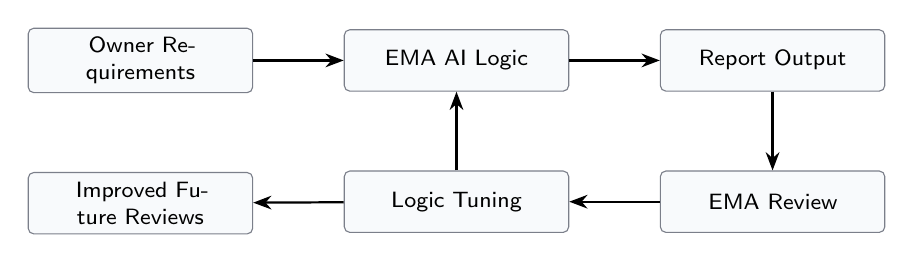
\begin{tikzpicture}[node distance=1.0cm and 1.15cm]
  \node[flowblock] (req) {Owner Requirements};
  \node[flowblock, right=of req] (logic) {EMA AI Logic};
  \node[flowblock, right=of logic] (output) {Report Output};
  \node[flowblock, below=of output] (review) {EMA Review};
  \node[flowblock, below=of logic] (tune) {Logic Tuning};
  \node[flowblock, below=of req] (improve) {Improved Future Reviews};
  \draw[arrow] (req) -- (logic);
  \draw[arrow] (logic) -- (output);
  \draw[arrow] (output) -- (review);
  \draw[arrow] (review) -- (tune);
  \draw[arrow] (tune) -- (logic);
  \draw[arrow] (tune) -- (improve);
\end{tikzpicture}
\end{center}

The review loop can tune:

\begin{itemize}
  \item requirement type definitions,
  \item evidence expectations,
  \item scoring weights,
  \item status thresholds,
  \item model-closeable classification,
  \item discipline-specific priorities,
  \item next action templates,
  \item taxonomy matrix entries,
  \item reviewer-facing phrasing.
\end{itemize}

\keyconcept{\strong{Loop summary:} Owner Requirements \flowarrow EMA AI Logic \flowarrow Report Output \flowarrow EMA Review \flowarrow Logic Tuning \flowarrow Improved Future Reviews}

% ============================================================
% 19. Current MVP vs planned intelligence
% ============================================================
\section{Current MVP vs Planned Intelligence}

\small
\begin{longtable}{p{1.4in}p{0.95in}p{0.95in}p{0.95in}p{2.45in}}
\caption{Capability status matrix}\\
\toprule
\textbf{Capability} & \textbf{Current MVP} & \textbf{In Progress} & \textbf{Planned} & \textbf{Notes} \\
\midrule
\endhead
Revit export & Yes & - & - & EMAExtractor exports structured model evidence. \\
Owner requirements ingest & Yes & - & - & Workbook rows are normalized and project-bound. \\
Evidence candidates & Yes & Yes & - & Deterministic resolver builds candidate evidence only. \\
Readiness scoring & Yes & Yes & - & Backend readiness is deterministic; report-side heuristic is also present. \\
Report generation & Yes & Yes & - & HTML report includes traceability, hidden JSON, and filters. \\
Ask EMA AI & Yes & Yes & - & Grounded on the hidden report context. \\
AI audit & Yes & Yes & - & Taxonomy and audit tabs surface review controls. \\
Taxonomy tuning & Partial & Yes & Yes & Current classifier exists; broader taxonomy expansion remains ongoing. \\
Drawing/spec evidence & Partial & Yes & Yes & Required for many high-risk requirement types. \\
Dashboard/Revit feedback loop & Partial & Yes & Yes & Optional dashboard sync and Revit-first workflow coexist. \\
Code compliance as an autonomous claim & No & - & No & Deliberately not claimed. \\
Enterprise Azure path & Partial & Yes & Yes & Future pilot path, not a claim of production deployment. \\
\bottomrule
\end{longtable}
\normalsize

\subsection{Scope labels}

\begin{itemize}
  \item \textbf{Current MVP} = implemented and available in the repository.
  \item \textbf{In progress} = partially implemented or actively being tuned.
  \item \textbf{Planned} = described in the repository as future or roadmap work.
  \item \textbf{Out of scope for current claims} = explicitly not promised as current production capability.
\end{itemize}

% ============================================================
% 20. Customer-facing guardrails
% ============================================================
\section{Customer-Facing Guardrails}

This section is intentionally prominent. The product must stay trustworthy.

\guardrailbox{\strong{EMA AI is not final compliance certification.}}
\guardrailbox{\strong{EMA AI is not a replacement for a licensed engineer or qualified reviewer.}}
\guardrailbox{\strong{Not all requirements are model-closeable.}}
\guardrailbox{\strong{Model evidence may be incomplete, stale, or absent.}}
\guardrailbox{\strong{Drawings, specifications, and manual review are often required.}}
\guardrailbox{\strong{AI only explains the available report context.}}
\guardrailbox{\strong{Candidate evidence requires human acceptance.}}
\guardrailbox{\strong{Tuning is expected and supported.}}

\subsection{Practical interpretation}

The safest way to read the report is as a first-pass evidence review. The report highlights what appears supported, what is still missing, and where human attention should go first. It does not replace project leadership or licensed engineering judgment.

% ============================================================
% 21. Worked examples
% ============================================================
\section{Worked Examples}

The examples below are intentionally practical and aligned with the repository's common evidence patterns.

\small
\begin{longtable}{p{0.85in}p{1.0in}p{1.2in}p{1.2in}p{1.15in}p{1.0in}}
\caption{Worked examples of requirement review behavior}\\
\toprule
\textbf{Topic} & \textbf{Validation type} & \textbf{Expected evidence} & \textbf{Available evidence} & \textbf{Status behavior} & \textbf{Why} \\
\midrule
\endhead
Panel / circuit & Model & Panel, Circuit Number, Supply From & Electrical fixtures exist, but some values are missing. & Not Met or Needs Human Review & Directly testable from model parameters. \\
Manufacturer / product & Specification & Manufacturer, model number, submittal, spec section & Family name hints exist but manufacturer metadata may be incomplete. & Needs Human Review & Category presence is context, not brand proof. \\
Plumbing / RPZ & Hybrid & Plumbing fixture/accessory, zone, location, spec or drawing proof & Fixtures exist, but coverage rules need external proof. & Needs Human Review & The model can prove presence, not coverage logic. \\
Controls / dryer vent & Hybrid or Specification & Controls schedule, sequence of operations, detail or field proof & Equipment exists, but control logic or termination details are absent. & Needs Human Review & The model cannot prove execution detail. \\
Grounding / tech & Model or Specification & Ground bar, bonding jumper, device data, panel, circuit, or spec evidence & Partial model context exists. & Needs Human Review unless direct evidence is explicit & Often needs parameter-level confirmation or external review. \\
Manual / drawing & Manual or Drawing & Sheet reference, coordination note, owner or reviewer sign-off & No direct model evidence exists. & Insufficient Model Data or Needs Human Review & The model is not the deciding artifact. \\
\bottomrule
\end{longtable}
\normalsize

\subsection{Interpretive notes}

\begin{itemize}
  \item A category match can raise confidence, but it does not close the requirement by itself.
  \item A candidate evidence list is a review queue, not a compliance certificate.
  \item High-risk language like manufacturer, controls, code, or field execution should trigger conservative handling.
\end{itemize}

% ============================================================
% 22. Glossary
% ============================================================
\section{Glossary}

\begin{longtable}{p{1.7in}p{4.95in}}
\caption{Key term glossary}\\
\toprule
\textbf{Term} & \textbf{Definition} \\
\midrule
\endhead
Owner Requirement & A client-supplied statement of expected project outcome or deliverable condition. \\
Requirement Type & The semantic family that determines expected evidence and closure rules. \\
Validation Type & The source and style of evidence required to review the requirement. \\
Model-Closeable & A requirement that can be fully evaluated from Revit model evidence alone, if the rule explicitly allows it. \\
Direct Closing Evidence & Evidence strong enough to close the requirement under the rule. \\
Supporting Context & Evidence that narrows the search but does not prove the requirement. \\
Missing Direct Evidence & The expected proof is not present or not captured. \\
Candidate Evidence & A possible match that still requires human acceptance. \\
Accepted Evidence & Candidate evidence that a reviewer has accepted. \\
Evidence Alignment & The degree to which available evidence matches the requirement's expected evidence profile. \\
Candidate Scope & The set of elements considered relevant enough to evaluate. \\
Key Issue Score & The prioritization score used to rank likely blockers. \\
Readiness & The deterministic health view for deliverable progression. \\
Next Best Action & The suggested next step for the reviewer or designer. \\
Taxonomy Matrix & The controlled map of requirement types, evidence expectations, and risks. \\
AI Audit & A control layer that highlights taxonomy gaps and false-positive risk. \\
RAG & Retrieval-augmented generation, used here only as a grounded assistant pattern over the report context. \\
Human-in-the-loop & A workflow where human review is part of the decision chain. \\
Report Context & The machine-readable report payload embedded in the HTML file. \\
EMAExtractor & The Revit add-in that exports, reviews, and launches the owner requirements workflow. \\
Revit Export & The structured evidence package generated from the model. \\
\bottomrule
\end{longtable}

% ============================================================
% 23. Technical field dictionary
% ============================================================
\section{Technical Field Dictionary}

The field dictionary below combines the most visible report fields with the backend fields that matter to reviewer traceability.

\begin{longtable}{p{1.45in}p{1.45in}p{3.35in}}
\caption{Compact field dictionary}\\
\toprule
\textbf{Field} & \textbf{Layer} & \textbf{Meaning} \\
\midrule
\endhead
\codepath{requirement_id} & Report / backend & Stable requirement identifier. \\
\codepath{source_row} & Report / backend & Workbook row number used for traceability. \\
\codepath{source_worksheet} & Report / backend & Worksheet from which the requirement was loaded. \\
\codepath{discipline} & Report / backend & Routing and scope label. \\
\codepath{requirement_text} & Report / backend & Canonical requirement statement. \\
\codepath{category} & Report / backend & Higher-level semantic context. \\
\codepath{owner_status} & Backend requirement & Source workbook status label. \\
\codepath{is_actionable} & Backend requirement & Whether the row participates in scoring. \\
\codepath{readiness_status} & Backend dashboard row & Readiness label for the current row. \\
\codepath{normalized_status} & Backend evidence row & Normalized evidence state. \\
\codepath{evidence_status} & Backend evidence row & Covered, missing, needs_review, blocked, not_applicable. \\
\codepath{evidence_review_status} & Backend evidence row & Candidate, accepted, rejected, needs_review, none. \\
\codepath{source_ref} & Backend evidence row & Evidence source reference string. \\
\codepath{evidence_type} & Backend evidence row & model, sheet, spec, manual, or hybrid. \\
\codepath{confidence} & Report / backend & Confidence score for the evidence or row. \\
\codepath{review_status} & Backend evidence row & Candidate/accepted/rejected status. \\
\codepath{rule_code} & Backend readiness action & Deterministic rule identifier. \\
\codepath{readiness_impact} & Backend readiness gap & Relative contribution to readiness. \\
\codepath{action_type} & Backend readiness action & Recommended action name. \\
\codepath{latest_export_id} & Backend readiness snapshot & Most recent completed export used in the snapshot. \\
\codepath{latest_sync_at} & Backend readiness snapshot & Timestamp of the latest completed sync. \\
\codepath{key_issue_score} & Report / backend & Prioritization score for the issue. \\
\codepath{candidate_scope_valid} & Report / add-in & Whether candidate scope remained within guardrails. \\
\codepath{full_model_fallback_used} & Report / add-in & Whether the resolver had to broaden beyond scoped search. \\
\bottomrule
\end{longtable}

% ============================================================
% 24. Diagrams appendix
% ============================================================
\section{Diagram Appendix}

\subsection{Diagram 1: Revit-first workflow}

\begin{center}
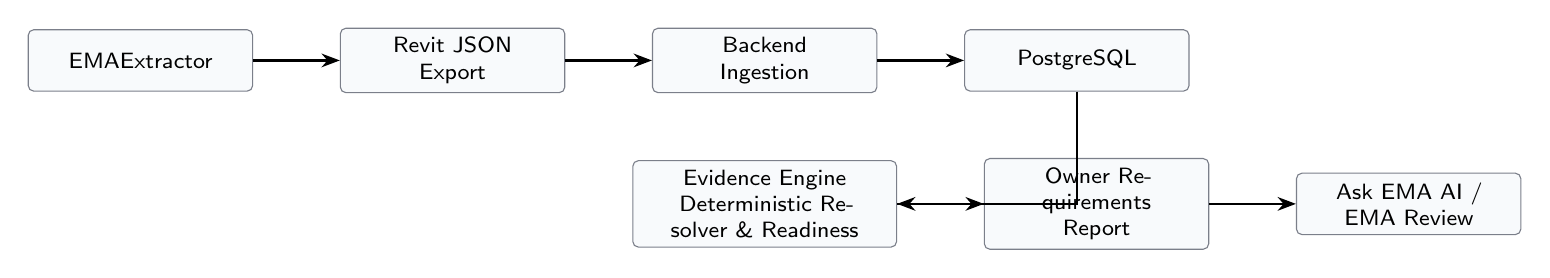
\begin{tikzpicture}[node distance=0.85cm and 1.1cm]
  \node[flowblock] (a) {EMAExtractor};
  \node[flowblock, right=of a] (b) {Revit JSON\\Export};
  \node[flowblock, right=of b] (c) {Backend\\Ingestion};
  \node[flowblock, right=of c] (d) {PostgreSQL};
  \node[flowwide, below=of c] (e) {Evidence Engine\\Deterministic Resolver \& Readiness};
  \node[flowblock, right=of e] (f) {Owner Requirements\\Report};
  \node[flowblock, right=of f] (g) {Ask EMA AI /\\EMA Review};
  \draw[arrow] (a) -- (b);
  \draw[arrow] (b) -- (c);
  \draw[arrow] (c) -- (d);
  \draw[arrow] (d) |- (e);
  \draw[arrow] (e) -- (f);
  \draw[arrow] (f) -- (g);
\end{tikzpicture}
\end{center}

\subsection{Diagram 2: Requirement review flow}

\begin{center}
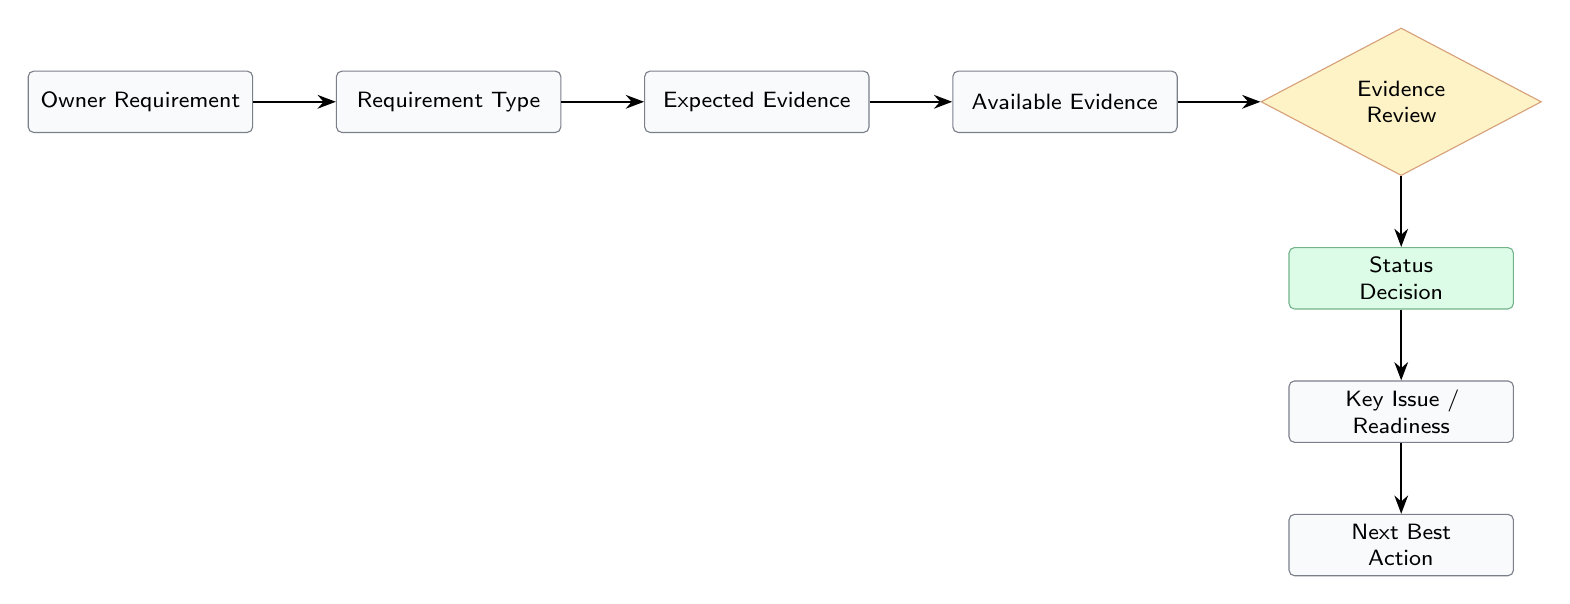
\begin{tikzpicture}[node distance=0.9cm and 1.05cm]
  \node[flowblock] (r) {Owner Requirement};
  \node[flowblock, right=of r] (t) {Requirement Type};
  \node[flowblock, right=of t] (x) {Expected Evidence};
  \node[flowblock, right=of x] (y) {Available Evidence};
  \node[flowdecision, right=of y] (z) {Evidence\\Review};
  \node[flowresult, below=of z] (s) {Status\\Decision};
  \node[flowblock, below=of s] (k) {Key Issue /\\Readiness};
  \node[flowblock, below=of k] (n) {Next Best\\Action};
  \draw[arrow] (r) -- (t);
  \draw[arrow] (t) -- (x);
  \draw[arrow] (x) -- (y);
  \draw[arrow] (y) -- (z);
  \draw[arrow] (z) -- (s);
  \draw[arrow] (s) -- (k);
  \draw[arrow] (k) -- (n);
\end{tikzpicture}
\end{center}

\subsection{Diagram 3: Evidence ladder}

\begin{center}
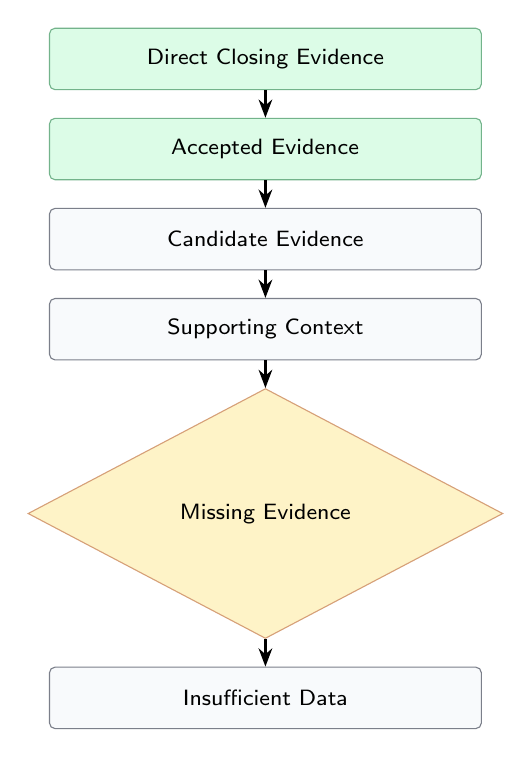
\begin{tikzpicture}[node distance=0.35cm]
  \node[flowresult, text width=5.25cm] (d1) {Direct Closing Evidence};
  \node[flowresult, below=of d1, text width=5.25cm] (d2) {Accepted Evidence};
  \node[flowblock, below=of d2, text width=5.25cm] (d3) {Candidate Evidence};
  \node[flowblock, below=of d3, text width=5.25cm] (d4) {Supporting Context};
  \node[flowdecision, below=of d4, text width=5.25cm] (d5) {Missing Evidence};
  \node[flowblock, below=of d5, text width=5.25cm] (d6) {Insufficient Data};
  \draw[arrow] (d1) -- (d2);
  \draw[arrow] (d2) -- (d3);
  \draw[arrow] (d3) -- (d4);
  \draw[arrow] (d4) -- (d5);
  \draw[arrow] (d5) -- (d6);
\end{tikzpicture}
\end{center}

\subsection{Diagram 4: Tuning loop}

\begin{center}
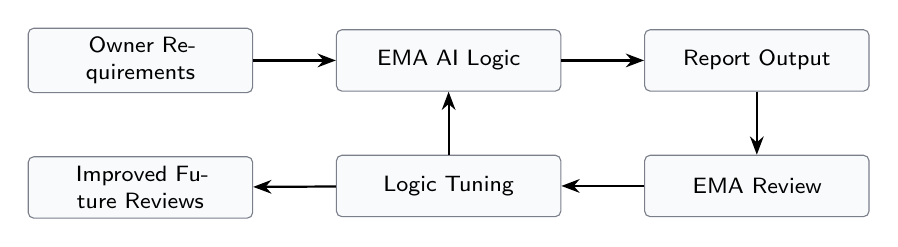
\begin{tikzpicture}[node distance=0.8cm and 1.05cm]
  \node[flowblock] (u1) {Owner Requirements};
  \node[flowblock, right=of u1] (u2) {EMA AI Logic};
  \node[flowblock, right=of u2] (u3) {Report Output};
  \node[flowblock, below=of u3] (u4) {EMA Review};
  \node[flowblock, below=of u2] (u5) {Logic Tuning};
  \node[flowblock, below=of u1] (u6) {Improved Future Reviews};
  \draw[arrow] (u1) -- (u2);
  \draw[arrow] (u2) -- (u3);
  \draw[arrow] (u3) -- (u4);
  \draw[arrow] (u4) -- (u5);
  \draw[arrow] (u5) -- (u2);
  \draw[arrow] (u5) -- (u6);
\end{tikzpicture}
\end{center}

% ============================================================
% Closing notes
% ============================================================
\section*{Closing Notes}

\begin{tcolorbox}[colback=white]
\small
\textbf{Practical readout:} EMA AI is most valuable when it is honest about the evidence it has, the evidence it lacks, and the evidence that still requires professional review. That is the core design choice behind the owner requirements report, the Revit navigator, the hidden report context, and the human-in-the-loop tuning loop.

\vspace{4pt}
\textbf{Repository truth:} the add-in report, the backend readiness snapshot, the taxonomy matrix, and the Ask EMA AI surface are related but distinct. The paper should reflect that distinction rather than flattening everything into one score.
\end{tcolorbox}

\vfill
\begin{center}
\muted{End of framework document}
\end{center}

\end{document}
